\documentclass{bioinfo}
\copyrightyear{2016} \pubyear{XXXX}

\access{Advance Access Publication Date: Day Month Year}
\appnotes{Application Note}


%\usepackage{tikz}
\usepackage{nicefrac}
\usepackage{comment}
\usepackage{color}

\usepackage{soul}
\sethlcolor{red}

\usepackage{graphicx}
\graphicspath{{./figures/}{./}}

%\usepackage{xr}
%\externaldocument{si-node.dating}

\usepackage{float}

\newcommand{\code}[1]{{\tt #1}}

\newcommand{\edit}[1]{\hl{#1}}

\begin{document}
\firstpage{1}

\subtitle{}

\title[node.dating]{node.dating: dating ancestors in phylogenetic trees in R}
\author[Jones \textit{et~al}.]{Bradley R. Jones\,$^{\text{\sfb 1, 2,}*}$ and Art F. Y. Poon\,$^{\text{\sfb 2,3}}$}
\address{$^{\text{\sf 1}}$Faculty of Health Sciences, Simon Fraser University, Burnaby, V5A 1S6, Canada, \\
$^{\text{\sf 2}}$BC Centre for Excellence in HIV/AIDS, Vancouver, V6Z 1Y6, Canada and \\
$^{\text{\sf 2}}$Department of Medicine, University of British Columbia, V5Z 1M9, Canada}

\corresp{$^\ast$To whom correspondence should be addressed.}

\history{Received on XXXXX; revised on XXXXX; accepted on XXXXX}

\editor{Associate Editor: XXXXXXX}

\abstract{
\textbf{Summary:}
Phylogenetic trees encode the evolutionary distances between species or populations.
With sufficient information, these evolutionary distances can be rescaled over time to provide estimates of the dates of the most recent ancestors of the species.
Here we present the \emph{R} program \code{node.dating}, \edit{divergence-time analysis software},  which uses a maximum likelihood method to estimate the dates of the internal nodes of a phylogenetic tree. \\
\textbf{Availability and Implementation:}
%\code{node.dating} is written in $R$ and requires the $R$ package, \emph{ape}.
\code{node.dating} is available as a part of the \emph{R} \edit{v3.30} package \emph{ape} \edit{v3.6} (cran.r-project.org).
\edit{{\tt node.dating} is also available in the GitHub repository: } https://github.com/brj1/node.dating\edit{, along with supplementary software and tests.}  \\
\textbf{Contact:} \href{brj1@sfu.ca}{brj1@sfu.ca}\\
\textbf{Supplementary information:} Supplementary data are available at \textit{Bioinformatics} online.}

\maketitle

%Keywords: 
%Phylogenetics, Ancestor Dating, Linear Regression, Molecular Clock \\

\underline{}

\vspace*{-25pt}

\section{Introduction} \label{sec:intro}
Phylogenetic trees represent the evolutionary relationships among populations or species through their common ancestors.  
%(Ways to make trees \citep{Raxml14}).
The length of a branch in the phylogeny usually corresponds to the expected amount of evolution between the ancestor and its descendant, where the passage of time and the rate of evolution are confounded.
However, when there is external information available on the location of nodes in the tree in time, then the branch lengths can be rescaled with respect to time given sufficient variation in node timings for measurable evolution to occur.
%In the presence of a molecular clock, the edges of a phylogenetic tree can be scaled over time to give a `time tree'.
%The nodes of a time tree also carry a time value which for the tips of the tree represent the sampling time of the tip's sequence.
Thus, the internal nodes of a time-scaled tree estimate the dates that the respective lineages diverged from their common ancestor \citep{Kumar16}.
These date estimates are an important resource for reconstructing the evolutionary history of species \citep{Shapiro04}.
In molecular epidemiology, these dates can also provide a rough approximation of transmission times during an outbreak of infectious disease 
\citep{Ypma13}.

A multitude of \edit{divergence-time analysis} software has been developed to reconstruct ancestral dates and create time-scaled trees using various techniques such as: linear regression \citep{Tempest}, maximum likelihood \citep{TipDates, r8ts, PAML}, Bayesian analysis \citep{BEAST}, heuristics \citep{UPGMA, TREBLE}, and least squares \citep{LSD}.
However, most of these software are either no longer actively maintained, difficult to obtain, or difficult to integrate into automated workflows.
Our software, \code{node.dating}, uses a maximum likelihood approach to date the internal nodes of a phylogenetic tree.
\code{node.dating} is written in \emph{R} \edit{v3.30} and is a recent addition to the \emph{R} package \emph{ape} \edit{v3.6} \citep{APE}.
%; it is also available in the GitHub repository: https://github.com/brj1/node.dating.
Previously, \emph{ape} had the capability to estimate the dates of internal nodes via the \code{chronos} function; however \code{chronos} requires ultrametric trees and is thus unable to incorporate information from tips that are sampled at different points in time.

\vspace*{-18pt}

\section{Algorithm} \label{sec:alg}
We start with a rooted phylogenetic tree with edge lengths measured in evolutionary distances and tips \edit{with heterochronous} dates.
A simple linear regression is used to estimate the rate of evolution assuming a strict molecular clock.
To estimate the dates of the internal nodes, we follow an approach described by \cite{Felsenstein81} and motivated by \emph{TipDates} \citep{TipDates}.
A maximum likelihood method is applied locally to date each internal node.
Then using these estimates, the algorithm iterates a specified number of times.

\vspace*{-18pt}

\section{Runtime and accuracy} \label{sec:tests}
In order to test the viability of \code{node.dating}, we ran it on 50 simulated trees with 100 tips each \edit{and simulated time span around 2400 days, similar to real within-patient HIV sequences.}
%All trees were rooted using the same root-to-tip method prior to date estimation using the different methods.
%We evaluated the results using a weighted root mean squared error (RMSE).
We compared these internal node dating results against a modified version of \emph{TempEst} v1.5 and \emph{LSD} 0.2 using \edit{a} weighted root mean squared error (RMSE).
\emph{TempEst} uses the prediction given by a linear regression to estimate the dates of the internal nodes and \emph{LSD} uses a least squares method.
We also compared our results with \emph{BEAST} v2.3.2 \edit{with a birth death skyline serial prior (Stadler et~al., 2013) and a strict clock model} using simulated sequence data as its inputs.
\edit{The simulation method and weighted RMSE} are detailed in the Supplementary Information.

\edit{The RMSE of {\tt node.dating} converged within 1 unit of its optimum RMSE of $22.1$ within 100 steps.
This quick convergence appears to be independant of data size as can be seen in supplementary trials found on the GitHub repository, https://github.com/brj1/node.dating.}
%The average weighted RMSE of the MRCA using \emph{TempEst} was $132.$ days and using \emph{LSD} was $24.9$ days.
The\edit{ }RMSE\edit{} of \emph{TempEst} \edit{was} higher than that obtained by \code{node.dating} with \edit{any number of} steps\edit{.}
%Overall, the RMSE of each tree using \code{node.dating} with 1000 iterations was less than the RMSE using \emph{TempEst}, suggesting that \code{node.dating} is more accurate at dating the internal nodes of phylogenetic trees.
However, The main purpose of \emph{TempEst} is to detect or verify the presence of a strict molecular clock, not to date internal nodes.
%We did not use \emph{TempEst} or \emph{LSD}'s root-to-tip regression in our experiments because we merely wanted to compare the internal node dating.
\edit{The RSME of \emph{LSD} was similar to {\tt node.dating} with 1000 steps, however {\tt node.dating} still performed better.
\emph{LSD} completed very quickly and remains a viable software for time-divergence analysis.
The advantage of {\tt node.dating} is the ease that it can be intergrated into \emph{R} pipelines.}
\emph{BEAST} performed the best of all methods when running $10^6$ steps, but this also took the most time.
In contrast, \emph{BEAST} performed poorly when limited to $10^4$ steps, requiring roughly the same amount of computing time as \code{node.dating} at 100 steps.
\edit{However, $10^4$ and even $10^6$ steps are extremely small amounts of iterations for a \emph{BEAST} run.
Furthermore}, results using \emph{BEAST} are not strictly comparable since we used sequence data as inputs instead of the phylogenetic trees.

\begin{table}[t]
	\caption[Runtime and accuracy]{The runtime and accuracy of \code{node.dating} and comparable software on 50 simulated trees\edit{. Runtime is in seconds and RMSE is in simulated days (see Supplementary Infornation)} }
	\label{tab:runtime}
	\centering
	\begin{tabular}{lrr}
		\hline
		Software & Runtime\edit{ } & RMSE\edit{ } \\
		\hline
		\code{node.dating} (initial) & 1.64 & 29.2 \\
		\code{node.dating} (1 step) & 2.26 & 26.7 \\
		\code{node.dating} (10 steps) & 7.62 & 23.7 \\
		\code{node.dating} (100 steps) & 62.1 & 22.8 \\
		\code{node.dating} (1000 steps) & 596.0 & 22.6 \\
		\code{node.dating} ($10^4$ steps) & 5950 & 22.1 \\
		\emph{TempEst} & 11.2 & 132.0 \\
		\emph{LSD} & 0.707 & 24.9 \\
		\emph{BEAST} ($10^4$ steps) & 181 & 419. \\
		\emph{BEAST} ($10^6$ steps) & 6840 & 20.1 \\
%		\emph{Minimum} & & 2.02 \\
		\hline
	\end{tabular}
\end{table}

\vspace*{-18pt}

\section{\edit{Intra-patient HIV example}} \label{sec:vis}
In this section, we provide a visualization of sequence data using the estimated dates of internal nodes.
We retrieved \edit{heterochronous} intra-host patient-derived sequences from Patient 16617 on the LANL HIV database (http://www.hiv.lanl.gov/, accessed June 24, 2015).
This patient's sequence data was collected in \cite{Llewellyn06} as Patient 1180.
We reconstructed the sequences' phylogenetic tree using the method described in the Supplementary Information.
We \edit{ } estimated the dates of the internal nodes using \code{node.dating} with 1000 iterations. 
In Figure \ref{fig:pat16617}, we show the genetic distance from the root versus time og the internal nodes and sampled sequences.
%Finally we plotted the genetic distance from the root versus time of the internal nodes and the sampled sequences. 
%This plot is shown in Figure \ref{fig:pat16617}.

\vspace*{-18pt}

\section{Future work} \label{sec:discuss}
One drawback of our methodology is that it assumes that the phylogeny follows a strict molecular clock.
However, the local likelihood model can be extended to incorporate a variable molecular clock; future work would like to include this extension.
The molecular clock assumption implies that mutations are strictly additive over time, which is not true.
It may be possible to incorporate this `negative' evolution into the model.

\begin{figure}[b]
	\centering
	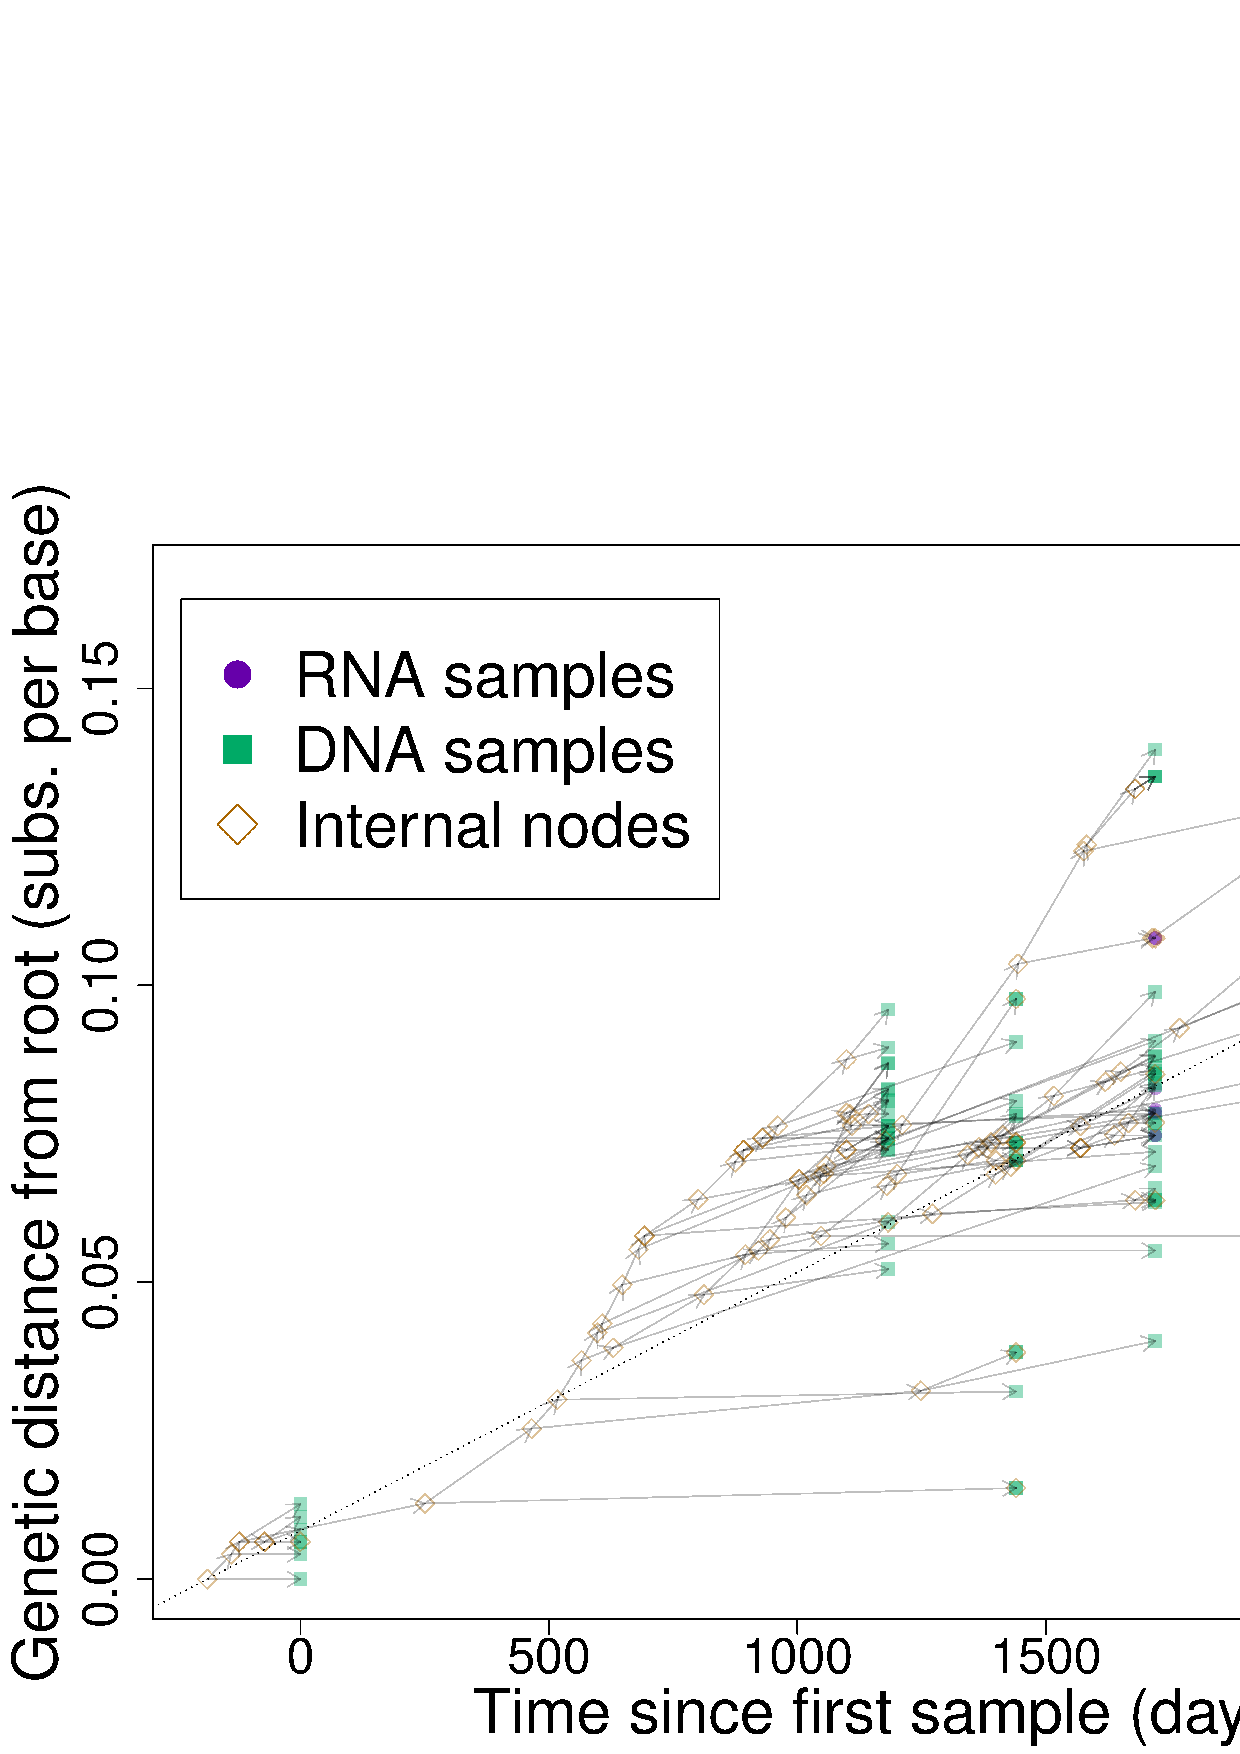
\includegraphics[width=\columnwidth]{patient_16617}
	\caption[Genetic distance versus time plot]{Genetic distance from the root versus time of the sequences from Patient 16617 from the LANL HIV database. The dates of the internal nodes were estimated using \code{node.dating} and are included in the plot. The edges between adjacent nodes of the tree are drawn as solid lines and the molecular clock is drawn by a dashed line.}
	\label{fig:pat16617}
\end{figure}

\vspace*{-18pt}

\section*{Acknowledgements} \label{sec:ackn}
We would like to thank Richard Liang for his aid in automating \emph{TempEst}.

\vspace*{-18pt}

\section*{Funding} \label{sec:fund}
This work was supported by the Canadian Institutes of Health Research (CIHR Team Grant: HIV Cure Research --- The Canadian HIV Cure Research Enterprise; CanCure), by a CIHR operating grant to AFYP (HOP-111406).
Research reported in this publication was partially supported by the Bill and Melinda Gates Foundation Award Number OPP1110049.
AFYP was supported by a CIHR New Investigator Award and by a salary award from the Michael Smith Foundation for Health Research, St.~Paul's Hospital Foundation and the Providence Health Care Research Institute.

\vspace*{-20pt}

\bibliographystyle{bio}
\begin{thebibliography}{14}
\providecommand{\natexlab}[1]{#1}
\providecommand{\url}[1]{\texttt{#1}}
\providecommand{\urlprefix}{URL }
\expandafter\ifx\csname urlstyle\endcsname\relax
  \providecommand{\doi}[1]{doi:\discretionary{}{}{}#1}\else
  \providecommand{\doi}{doi:\discretionary{}{}{}\begingroup
  \urlstyle{rm}\Url}\fi

\bibitem[{Drummond and Rodrigo(2000)}]{UPGMA}
Drummond, A. and Rodrigo, R., A~G (2000) Reconstructing genealogies of serial
  samples under the assumption of a molecular clock using serial-sample
  {UPGMA}.
\newblock \emph{Molecular Biology and Evolution}, 17(12), 1807--1815.

\bibitem[{Drummond and Rambaut(2007)}]{BEAST}
Drummond, A.~J. and Rambaut, A. (2007) {BEAST}: {Bayesian} evolutionary
  analysis by sampling trees.
\newblock \emph{BMC Evolutionary Biology}, 7, 214.

\bibitem[{Felsenstein(1981)}]{Felsenstein81}
Felsenstein, J. (1981) Evolutionary trees from {DNA} sequences: a maximum
  likelihood approach.
\newblock \emph{Journal of Molecular Evolution}, 17, 368--376.

\bibitem[{Kumar and Hedges(2016)}]{Kumar16}
Kumar, S. and Hedges, S.~B. (2016) Advances in time estimation methods for
  molecular data.
\newblock \emph{Molecular Biology and Evolution}, 33(4), 863--869.

\bibitem[{Llewellyn et~al.(2006)}]{Llewellyn06}
Llewellyn, N. et~al. (2006) Continued evolution of {HIV-1} circulating in blood
  monocytes with antiretroviral therapy: genetic analysis of {HIV-1} in
  monocytes and {CD4+} {T} cells of patients with discontinued therapy.
\newblock \emph{J Leukoc Biol}, 80(5), 1118--1126.

\bibitem[{Paradis et~al.(2004)}]{APE}
Paradis, E. et~al. (2004) {APE}: analyses of phylogenetics and evolution in {R}
  language.
\newblock \emph{Bioinformatics}, 20(2), 289--290.

\bibitem[{Rambaut(2000)}]{TipDates}
Rambaut, A. (2000) Estimating the rate of molecular evolution: incorporating
  non-contemporaneous sequences into maximum likelihood phylogenies.
\newblock \emph{Bioinformatics}, 16(4), 395--399.

\bibitem[{Rambaut et~al.(2016)}]{Tempest}
Rambaut, A. et~al. (2016) Exploring the temporal structure of heterochronous
  sequences using {TempEst} (formerly {Path-O-Gen}).
\newblock \emph{Virus Evolution}, 2, vew007.

\bibitem[{Sanderson(2003)}]{r8ts}
Sanderson, M.~J. (2003) {r8s}: inferring absolute rates of molecular evolution
  and divergence times in the absence of a molecular clock.
\newblock \emph{Bioinformatics}, 19(2), 301--302.

\bibitem[{Shapiro et~al.(2004)}]{Shapiro04}
Shapiro, B. et~al. (2004) Rise and fall of the {Beringian Steppe} bison.
\newblock \emph{Science}, 306, 1561--1565.

\bibitem[{Stadler et~al.(2013)}]{Stadler13}
\edit{Stadler, T. et~al. (2013) Birth-death skyline plot reveals temporal changes of epidemic spread in HIV and hepatitis C virus. (HCV).
\newblock \emph{PNAS}, 110(1), 228--33.}

\bibitem[{To et~al.(2016)}]{LSD}
To, T.-H. et~al. (2016) Fast dating using least-squares criteria and
  algorithms.
\newblock \emph{Systematic Biology}, 65(1), 82--97.

\bibitem[{Yang(2007)}]{PAML}
Yang, Y. (2007) {PAML} 4: phylogenetic analysis by maximum likelihood.
\newblock \emph{Molecular Biology and Evolution}, 24(8), 1585--1591.

\bibitem[{Yang et~al.(2007)}]{TREBLE}
Yang, Z. et~al. (2007) Tree and rate estimation by local evaluation of
  heterochronous nucleotide data.
\newblock \emph{Bioinformatics}, 23(2), 169--176.

\bibitem[{Ypma et~al.(2013)}]{Ypma13}
Ypma, R. J.~F. et~al. (2013) Relating phylogenetic trees to transmission trees
  of infectious disease outbreaks.
\newblock \emph{Genetics}, 195(3), 1055--1062.

\end{thebibliography}


\end{document}
